\begin{figure*}[t]
    \centering
    \begin{tikzpicture}
      \node[inner sep=0pt, anchor=south west] (uav) at (0,0)
        {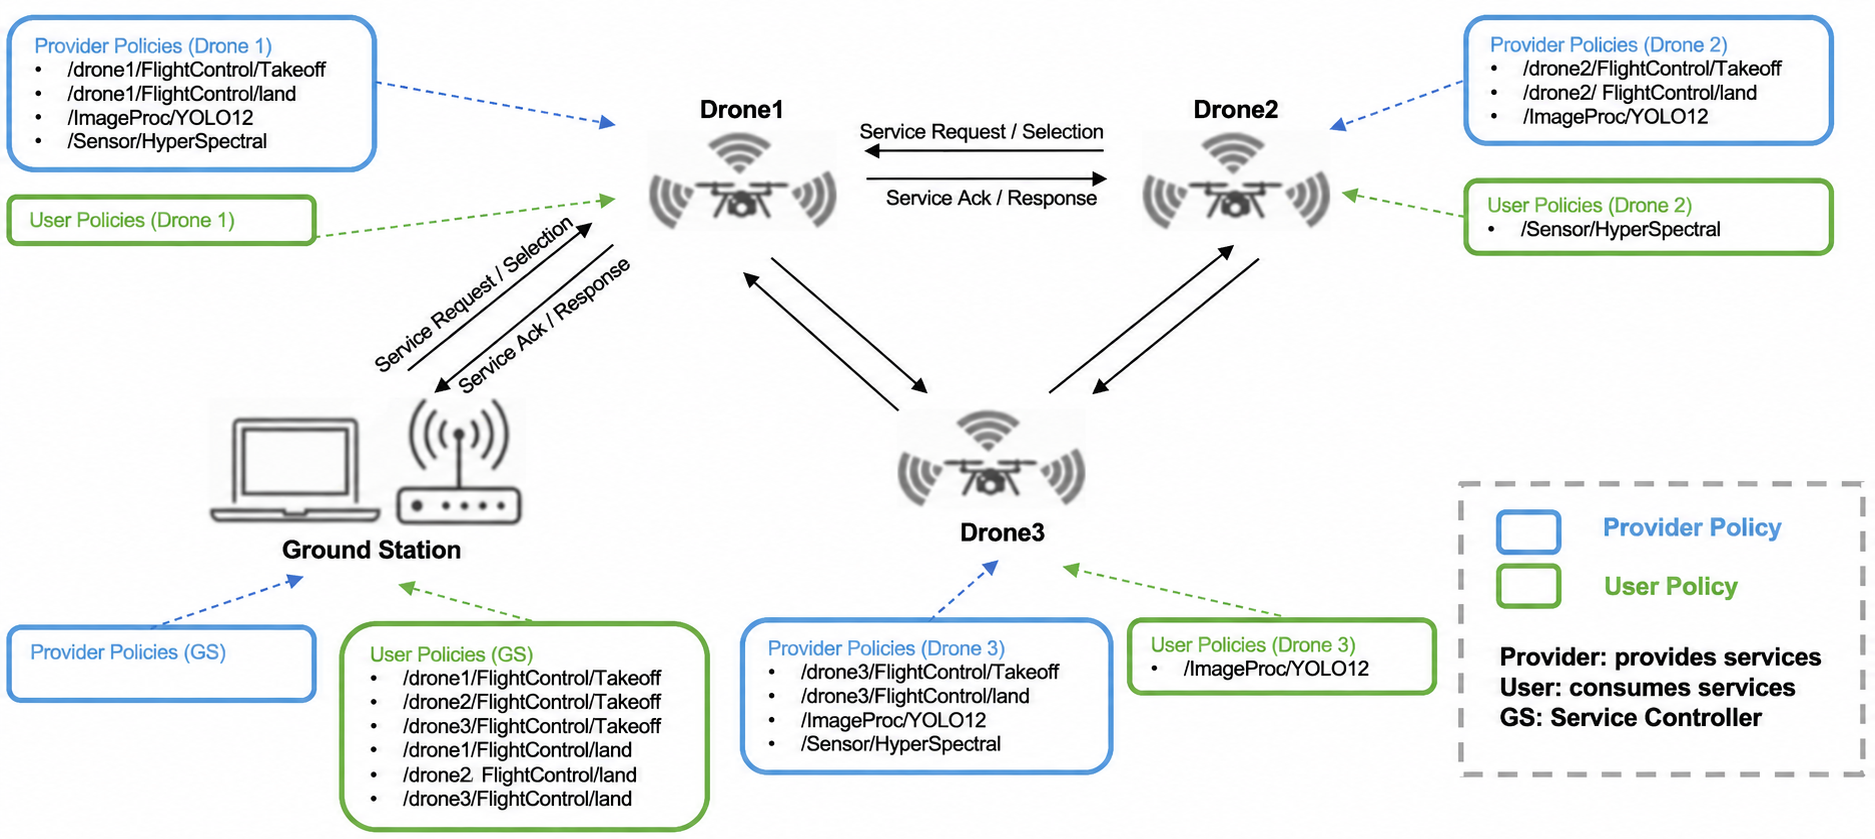
\includegraphics[width=.8\textwidth]{figures/drones-corrected.png}};
      \node[anchor=west, fill=white, inner sep=0pt,
        font=\sffamily\fontsize{5.2pt}{6pt}\selectfont]
        at ([xshift=.17\textwidth,yshift=14pt]uav.south west)
        {/drone2/FlightControl/land};
    \end{tikzpicture}
    \caption{UAV Network Application Example}
    \vspace{-3mm}
    \label{fig:UAV-NDNSF}
\end{figure*}

An NDN service framework should provide three core functions: (1) \textbf{service publication and discovery} mechanisms that enable providers to publish services and users to locate available services; (2) \textbf{access control mechanisms}, including authorization and enforcement, that regulate which entities may provide or access services; and (3) \textbf{service invocation mechanisms} that allow users to request services.

NDNSF combines \textbf{\emph{fine-grained access control}} and \textbf{\emph{dynamic provider selection}} in a \textbf{\emph{one-to-many service model}}. It uses NAC-ABE to control which entities may provide or access services. Under one ABE authority, an entity's service permissions can be encoded in a single decryption key (Section~\ref{sec:service-controller}). In the four-message invocation flow, authorized providers return ACKs indicating their willingness to execute the current task, optionally including resource information. The user combines this feedback with application-specific criteria to select one or more providers (Section~\ref{sec:provider-selection}). The user then shares the input decryption key only with the selected providers (Section~\ref{sec:messages}). Participation feedback thus guides provider selection, which determines access to the protected task input.
% (3) \textbf{security mechanisms} that ensure the integrity, authenticity, and confidentiality of service messages; and  
% and illustrate how our design choices support the following design goals:
%(a) \emph{Generality}: support diverse service types and adapt to varying application requirements;
%(b) \emph{Reliability}: tolerate failures and maintain service availability under adverse network conditions; and
%(c) \emph{Scalability}: accommodate new users and providers without complex configuration and significant performance degradation.

%\subsection{Design Assumptions}

%Given the distributed nature of the proposed service framework, we assume that candidate service providers are reachable at the network layer when service interactions are initiated. This assumption is consistent with prior NDN-based service designs and does not preclude temporary disconnections caused by mobility or network dynamics.

%In addition, as with all NDN applications, NDNSF assumes that participating entities have completed the standard NDN bootstrapping process. Specifically, each entity is expected to possess the necessary trust anchors, certificates, and trust schemas required to enable data-centric security and name-based trust verification.


\subsection{Design Overview}

In an NDNSF-based distributed application, \emph{Service Providers} process requests and generate responses, \emph{Service Users} issue requests and consume responses, and the \emph{Service Controller} authorizes providers and users and defines their service permissions.  Figure~\ref{fig:UAV-NDNSF} illustrates these interactions in a UAV network. Drones act as \emph{Service Providers} offering flight-control and peer services (e.g., image processing or sensing), while the ground station serves as a \emph{Service User}. The \emph{Service Controller} may reside on the ground station or a dedicated in-network server.

%To support the functionalities of these entities, NDNSF consists of four core functional modules:
%(1) \textbf{Service Provider Bootstrap}, which enables Service Providers to obtain from the Service Controller the services they are authorized to offer and the necessary NAC-ABE keys; 
%(2) \textbf{Service User Bootstrap}, which enables Service Users to obtain from the Service Controller the services they are authorized to access and the necessary NAC-ABE keys;
%(3) \textbf{Secure Service Communication}, which ensures authenticity, integrity, and confidentiality of service messages over NDN; and
%(4) \textbf{Provider Selection}, which manages interactions among multiple Service Providers using different selection strategies.

\subsection{Service Publication and Discovery}

NDNSF discovers candidate providers through the Request--ACK exchange, referred to here as \emph{task solicitation}. The user publishes a Request for the service name, optionally carrying a protected task descriptor, without preselecting a provider. Providers that pass the applicable authorization checks assess the request and return positive ACKs when willing to participate; reading a protected descriptor also requires matching ABE decryption capability. The user then selects providers from their feedback. The message formats and authorization checks are described in Section~\ref{sec:messages}.

\begin{figure}
    \centering
    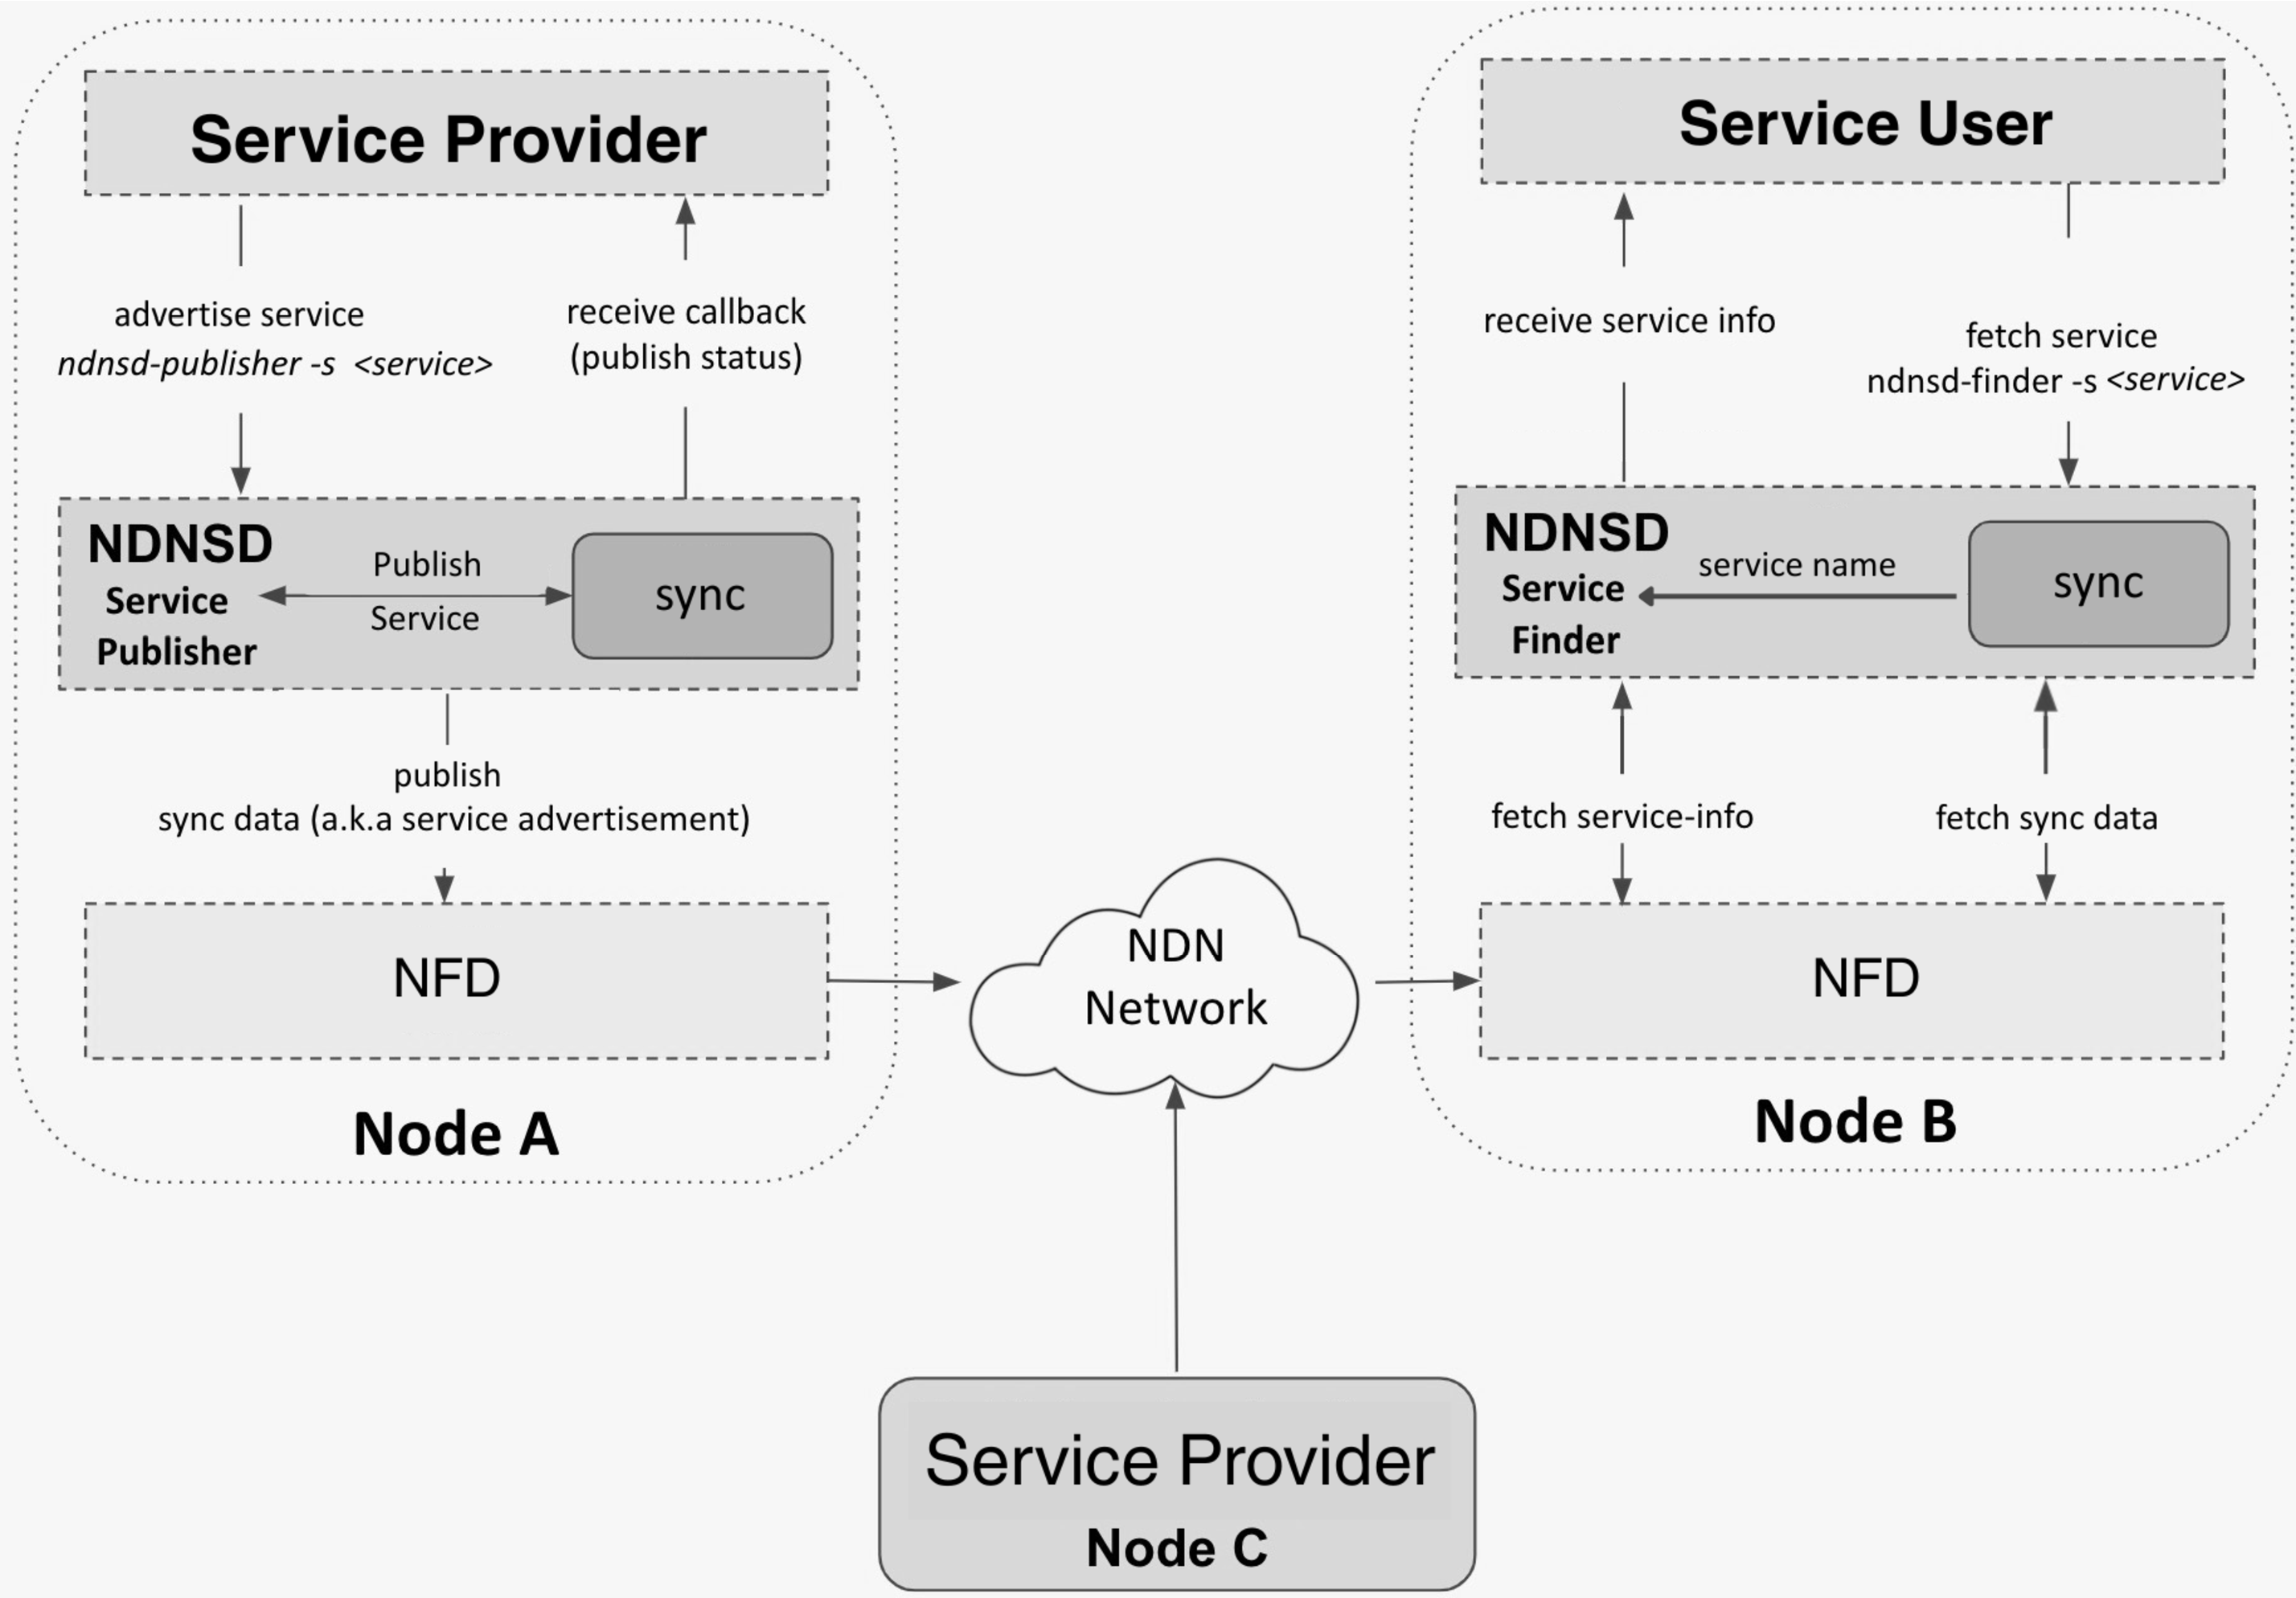
\includegraphics[width=\columnwidth]{figures/ndnsd.pdf}
    \caption{Service Publication and Discovery with NDNSD (adapted from~\cite{dulal2022ndnsd}, Fig.~2)}
    \vspace{-3mm}
    \label{fig:NDNSD}
\end{figure}

NDNSF can also use NDNSD~\cite{dulal2022ndnsd} to publish and discover service information before invocation. As shown in Figure~\ref{fig:NDNSD}, service providers publish their service information via NDN Sync (Section~\ref{sec:background}), allowing other participants in the Sync group (e.g., service users) to discover available services. NDNSD requires a service name and service-information lifetime; applications can add fields such as the provider's name prefix and a description. For example, a drone may publish the following information for its service:
\begin{quote}
Service Name: \texttt{/UAVNET/ImageProc/YOLO12}

Provider Name Prefix: \texttt{/UAVNET/drone2}

ServiceInfo Lifetime: \texttt{60s}

Description: \texttt{Real-time object detection service using YOLOv12}
\end{quote}
Advertisements help applications identify potential providers before issuing a request. Previously published information may remain retrievable from other available copies even when its provider is offline. However, an advertisement does not establish the provider's current availability or willingness to execute a particular task.

An application that has already chosen a provider can use targeted invocation (Section~\ref{sec:targeted-invocation}).

\subsection{Service Controller and Access Control}
\label{sec:service-controller}

\begin{figure*}[t]
\centering 

\begin{minipage}[c]{0.63\textwidth}
    \centering
    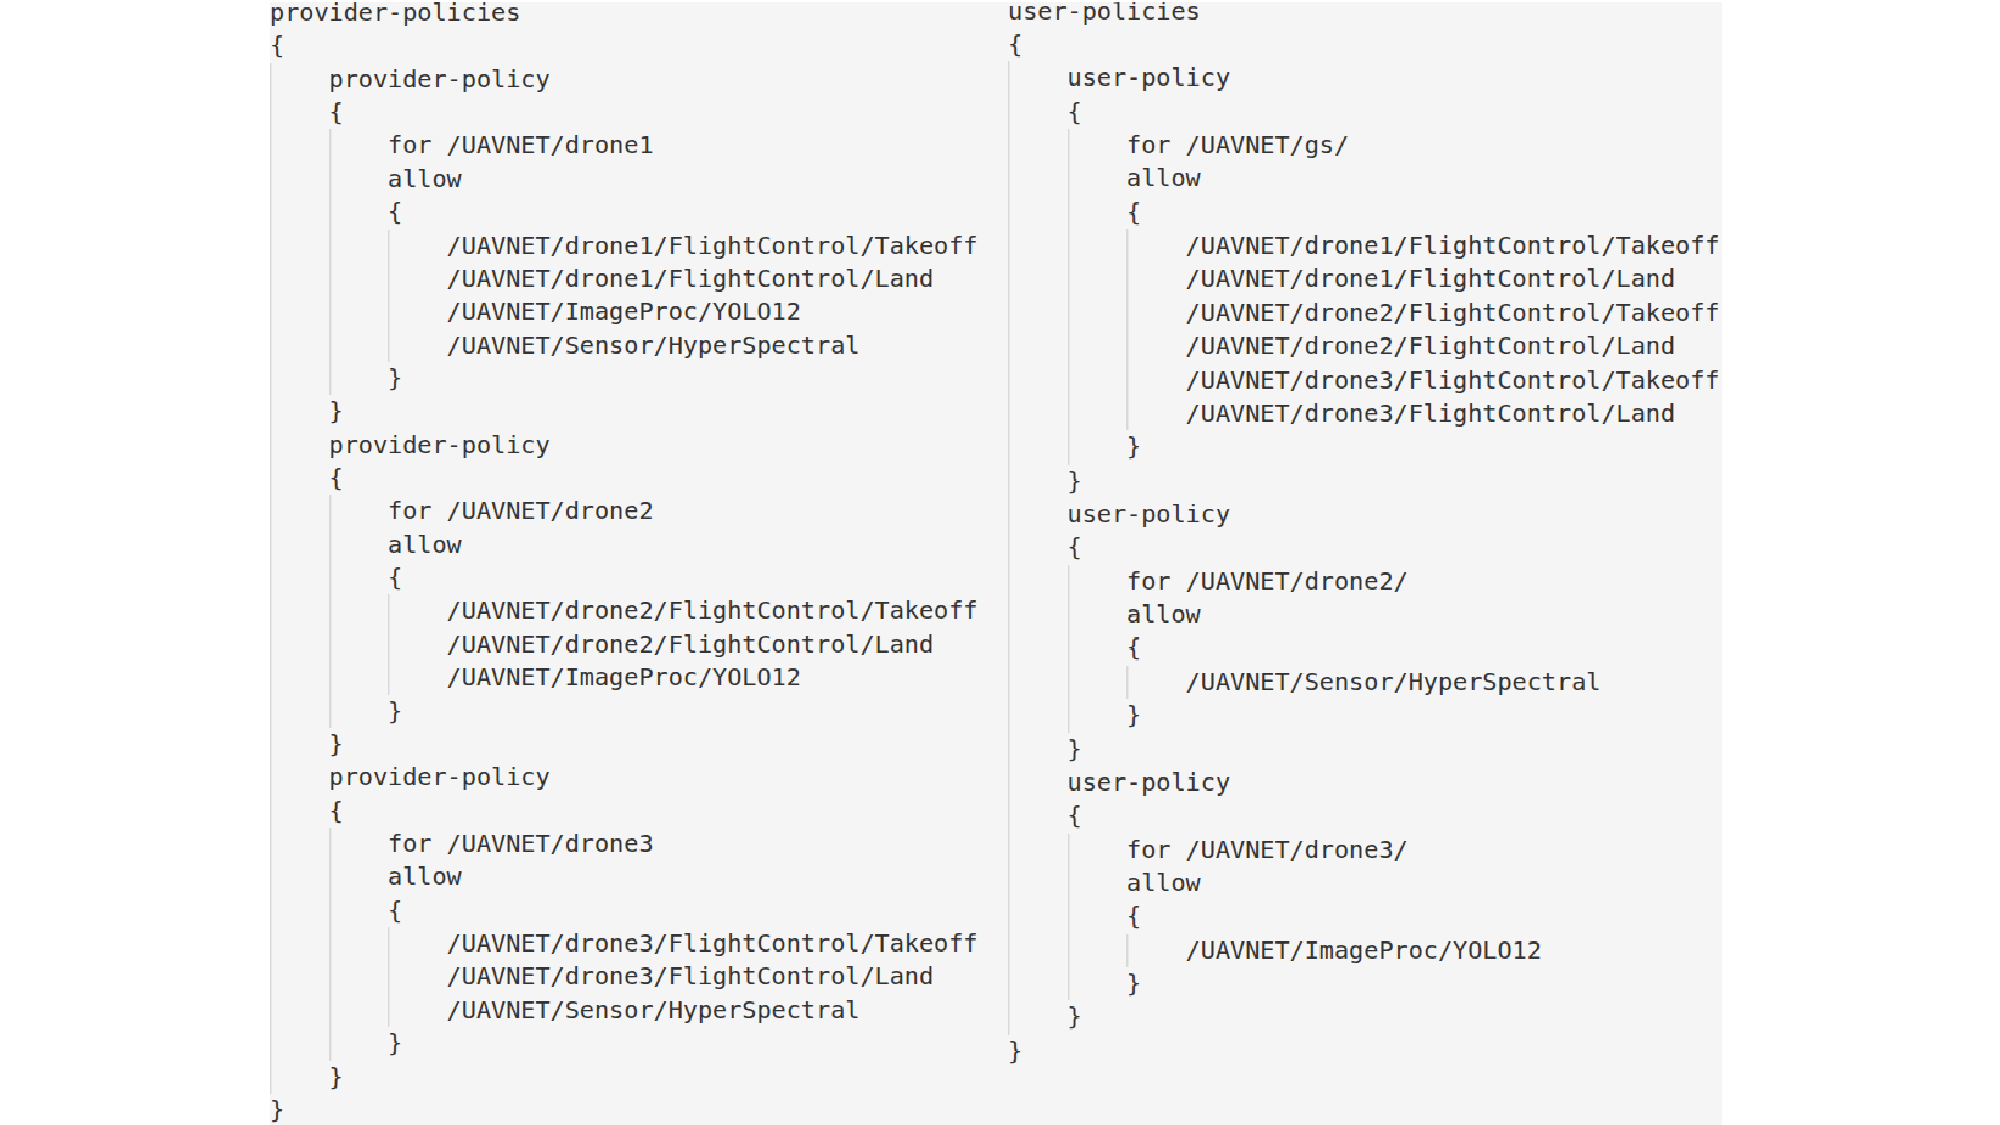
\includegraphics[width=\linewidth]{figures/user-provider-policy.pdf}
    \caption{An Example of Access Control Policies}
    \label{fig:PolicyExample}
\end{minipage}
\hfill
\begin{minipage}[c]{0.35\textwidth}
\centering

    % --- ROW 1: Request & ACK ---
    \begin{subfigure}[t]{0.49\linewidth}
    \centering
    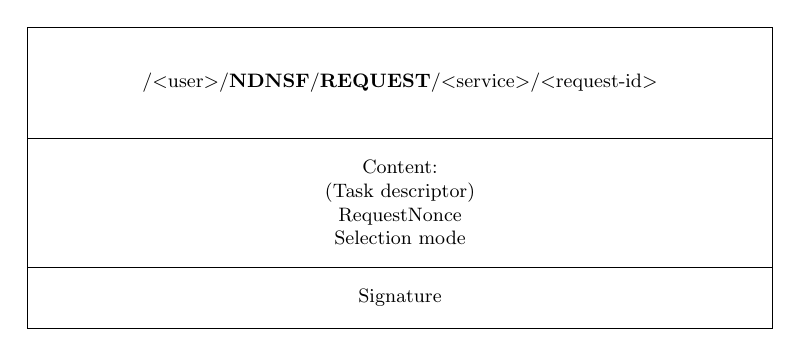
\begin{tikzpicture}[scale=0.78, transform shape]
    \def\W{1.0\linewidth} 
    \def\Hname{1.8}    % Vertically shrunk from 2.6
    \def\Hcontent{2.1} % Vertically shrunk from 2.2
    \def\Hsig{1.0}
    
    \useasboundingbox (0,0) rectangle (\W,\Hname+\Hcontent+\Hsig);
    \draw (0,0) rectangle (\W,\Hname+\Hcontent+\Hsig);
    \draw (0,\Hsig) -- (\W,\Hsig);
    \draw (0,\Hsig+\Hcontent) -- (\W,\Hsig+\Hcontent);
    
    \node[align=center, text width=0.95*\W, font=\small, inner sep=1pt] at (0.5*\W,\Hsig+\Hcontent+\Hname/2) {/$<$user$>$/\textbf{\allowbreak NDNSF}/\textbf{\allowbreak REQUEST}/\allowbreak $<$service$>$/\allowbreak $<$request-id$>$};
    \node[align=center, text width=0.95*\W, font=\small, inner sep=1pt] at (0.5*\W,\Hsig+\Hcontent/2) {Content:\\(Task descriptor)\\RequestNonce\\Selection mode};
    \node[font=\small] at (0.5*\W,\Hsig/2) {Signature};
    \end{tikzpicture}
    \caption{Request}
    \end{subfigure}%
    \hfill
    \begin{subfigure}[t]{0.49\linewidth}
    \centering
    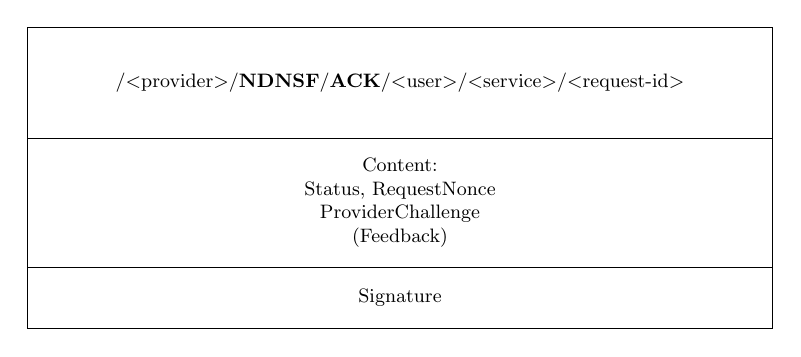
\begin{tikzpicture}[scale=0.78, transform shape]
    \def\W{1.0\linewidth}
    \def\Hname{1.8}    % Vertically shrunk from 2.6
    \def\Hcontent{2.1} % Vertically shrunk from 2.2
    \def\Hsig{1.0}
    
    \useasboundingbox (0,0) rectangle (\W,\Hname+\Hcontent+\Hsig);
    \draw (0,0) rectangle (\W,\Hname+\Hcontent+\Hsig);
    \draw (0,\Hsig) -- (\W,\Hsig);
    \draw (0,\Hsig+\Hcontent) -- (\W,\Hsig+\Hcontent);
    
    \node[align=center, text width=0.95*\W, font=\small, inner sep=1pt] at (0.5*\W,\Hsig+\Hcontent+\Hname/2) {/$<$provider$>$/\textbf{\allowbreak NDNSF}/\textbf{\allowbreak ACK}/\allowbreak $<$user$>$/\allowbreak $<$service$>$/\allowbreak $<$request-id$>$};
    \node[align=center, text width=0.95*\W, font=\small, inner sep=1pt] at (0.5*\W,\Hsig+\Hcontent/2) {Content:\\Status, RequestNonce\\ProviderChallenge\\(Feedback)};
    \node[font=\small] at (0.5*\W,\Hsig/2) {Signature};
    \end{tikzpicture}
    \caption{ACK}
    \end{subfigure}
    
    \vspace{6mm} 
    
    % --- ROW 2: Selection & Response ---
    \begin{subfigure}[t]{0.49\linewidth}
    \centering
    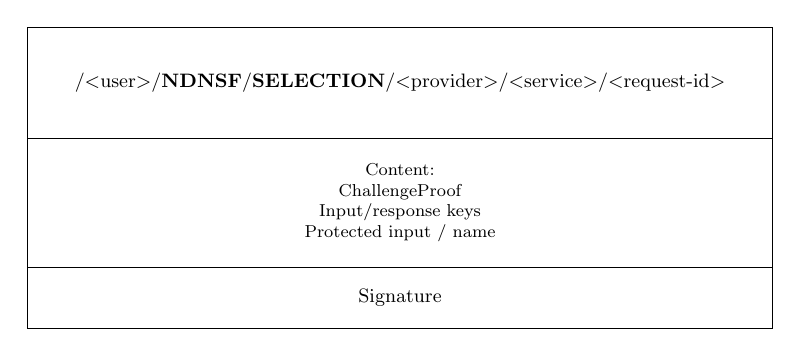
\begin{tikzpicture}[scale=0.78, transform shape]
    \def\W{1.0\linewidth}
    \def\Hname{1.8}    % Vertically shrunk from 2.6
    \def\Hcontent{2.1} % Vertically shrunk from 2.2
    \def\Hsig{1.0}
    
    \useasboundingbox (0,0) rectangle (\W,\Hname+\Hcontent+\Hsig);
    \draw (0,0) rectangle (\W,\Hname+\Hcontent+\Hsig);
    \draw (0,\Hsig) -- (\W,\Hsig);
    \draw (0,\Hsig+\Hcontent) -- (\W,\Hsig+\Hcontent);
    
    \node[align=center, text width=0.95*\W, font=\small, inner sep=1pt] at (0.5*\W,\Hsig+\Hcontent+\Hname/2) {/$<$user$>$/\textbf{\allowbreak NDNSF}/\textbf{\allowbreak SELECTION}/\allowbreak $<$provider$>$/\allowbreak $<$service$>$/\allowbreak $<$request-id$>$};
    \node[align=center, text width=0.95*\W, font=\footnotesize, inner sep=1pt] at (0.5*\W,\Hsig+\Hcontent/2) {Content:\\ChallengeProof\\Input/response keys\\Protected input / name};
    \node[font=\small] at (0.5*\W,\Hsig/2) {Signature};
    \end{tikzpicture}
    \caption{Selection}
    \end{subfigure}%
    \hfill
    \begin{subfigure}[t]{0.49\linewidth}
    \centering
    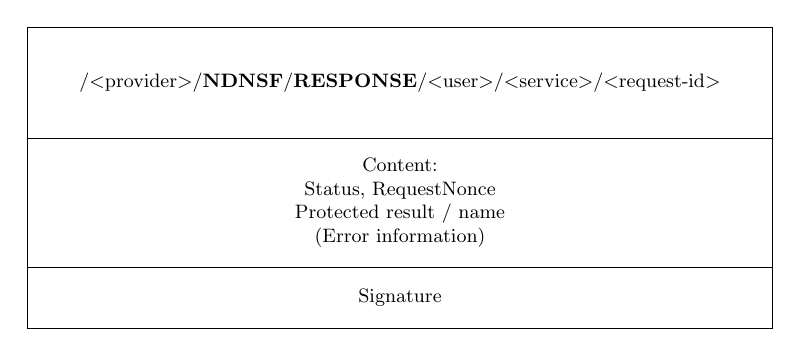
\begin{tikzpicture}[scale=0.78, transform shape]
    \def\W{1.0\linewidth}
    \def\Hname{1.8}    % Vertically shrunk from 2.6
    \def\Hcontent{2.1} % Vertically shrunk from 2.2
    \def\Hsig{1.0}
    
    \useasboundingbox (0,0) rectangle (\W,\Hname+\Hcontent+\Hsig);
    \draw (0,0) rectangle (\W,\Hname+\Hcontent+\Hsig);
    \draw (0,\Hsig) -- (\W,\Hsig);
    \draw (0,\Hsig+\Hcontent) -- (\W,\Hsig+\Hcontent);
    
    \node[align=center, text width=0.95*\W, font=\small, inner sep=1pt] at (0.5*\W,\Hsig+\Hcontent+\Hname/2) {/$<$provider$>$/\textbf{\allowbreak NDNSF}/\textbf{\allowbreak RESPONSE}/\allowbreak $<$user$>$/\allowbreak $<$service$>$/\allowbreak $<$request-id$>$};
    \node[align=center, text width=0.95*\W, font=\small, inner sep=1pt] at (0.5*\W,\Hsig+\Hcontent/2) {Content:\\Status, RequestNonce\\Protected result / name\\(Error information)};
    \node[font=\small] at (0.5*\W,\Hsig/2) {Signature};
    \end{tikzpicture}
    \caption{Response}
    \end{subfigure}

\caption{Principal fields of NDNSF's four invocation message types. ACK illustrates a positive reply; parentheses mark optional fields. Names are schematic; protection metadata and extensions are omitted.}
\label{fig:ndnsf-message-formats}
\end{minipage}
\end{figure*}


The \textbf{Service Controller} manages access control policies for providers and users. Provider policies specify which services an entity may offer, while user policies define which services it may access. These policies are designed to be simple and intuitive by leveraging NDN naming semantics. As shown on the left side of Figure~\ref{fig:PolicyExample}, drones 1-3 are authorized to provide their own flight-control services ending in \texttt{/FlightControl/Takeoff} and \texttt{/FlightControl/Land}. In addition, Drone~1 and Drone~2 may offer the image-processing service \texttt{/UAVNET/ImageProc/YOLO12}, while Drone~1 and Drone~3 may provide the sensing service \texttt{/UAVNET/Sensor/HyperSpectral}. The right side of the figure shows the corresponding user policies: the ground station \texttt{/UAVNET/gs} may access the flight-control services of all three drones, Drone~2 may access the hyperspectral sensing service, and Drone~3 may access the image-processing service.

Access control policies are translated into logical combinations of ABE attributes. NDNSF uses \textbf{service attributes} (\texttt{/SERVICE/<service-name>}) and \textbf{permission attributes} (\texttt{/PERMISSION/<service-name>}) to represent provisioning and access rights, respectively.  Here, \texttt{<service-name>} is a hierarchical NDN name consisting of one or more components that identify either a common service offered by multiple providers, a provider-specific service, or even a function within a service. These attributes encrypt service messages to control access (Section~\ref{sec:messages}). Under one ABE authority and the same set of public parameters, one DKEY can encode multiple service permissions. The naming hierarchy alone does not grant access to all services under a prefix; the ABE policy must encode the intended permissions.

\begin{figure}
    \centering
    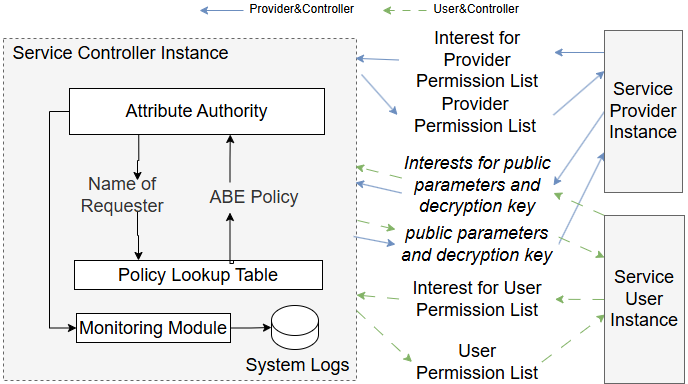
\includegraphics[width=.9\columnwidth]{figures/NDNSF_ServiceController.png}
    \caption{NDNSF Service Controller}
    \label{fig:ServiceController}
\end{figure}


%\begin{figure}[]
%\centering
%\begin{subfigure}[t]{0.25\textwidth}
%    \centering
%    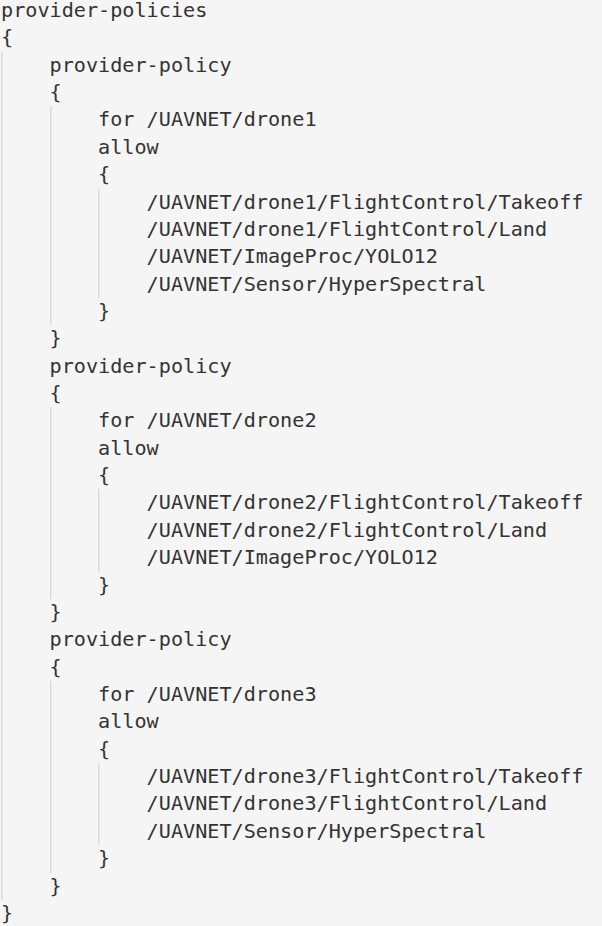
\includegraphics[width=\linewidth]{figures/Provider-policies.png}
%    \caption{Provider policies}
%\end{subfigure}
%\hfill
%\begin{subfigure}[t]{0.25\textwidth}
%    \centering
%    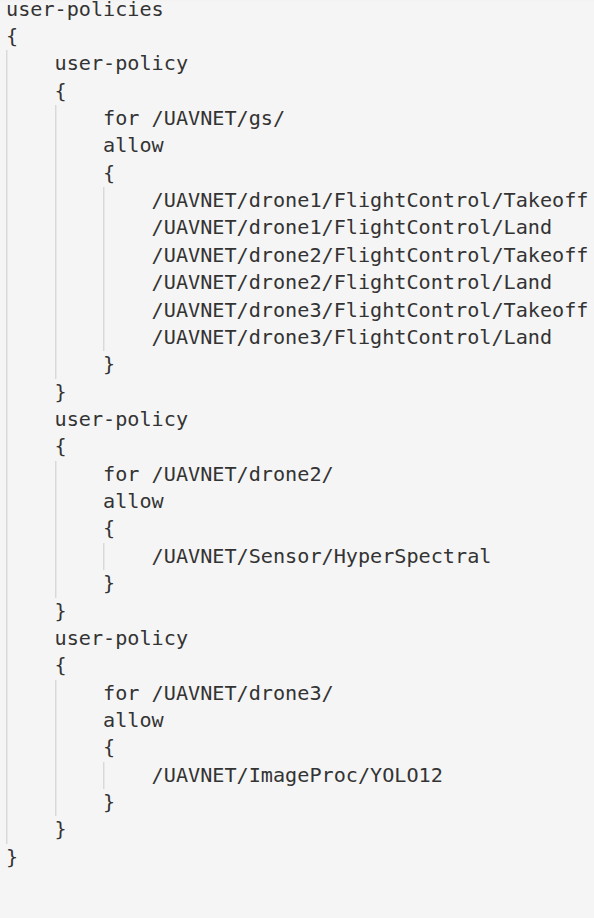
\includegraphics[width=\linewidth]{figures/User-policies.png}
%    \caption{User policies}
%\end{subfigure}
%\caption{An Example of Access Control Policies}
%\vspace{-3mm}
%\label{fig:PolicyExample}
%\end{figure}


The deployment administrator determines service permissions, and the Service Controller participates during onboarding and policy updates. As shown in Figure~\ref{fig:ServiceController}, inside the controller, the \textbf{Attribute Authority} maps an entity's name to its policy in the \textbf{Policy Lookup Table} and generates a decryption key (DKEY) that enables access to data encrypted under the corresponding attributes. The controller then securely distributes each entity's DKEY encrypted with the entity's public key. Through Interest--Data exchanges, users retrieve from the controller a \emph{User Permission List} specifying accessible services, while providers retrieve a \emph{Provider Permission List} specifying the services they are authorized to offer.

%Overall, NDNSF enables fine-grained, name-based access control over both service providers and users. By combining ABE with hierarchical NDN names, NDNSF achieves greater flexibility and scalability than traditional RBAC systems, while requiring only a single DKEY per entity regardless of the number of permissions.

\begin{comment}
\subsection{Service Provider and User}

\begin{figure}
    \centering
    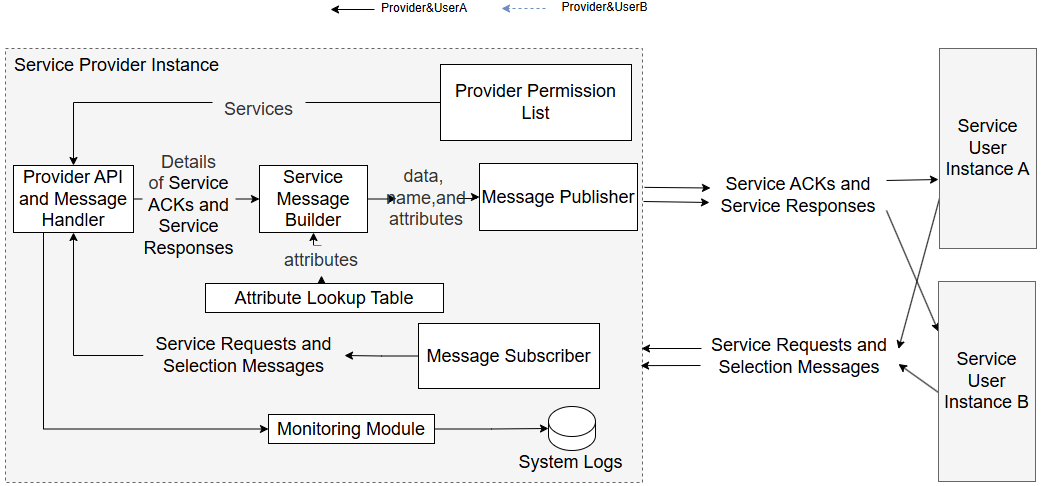
\includegraphics[width=\columnwidth]{figures/NDNSF_ServiceProvider.png}
    \caption{NDNSF Service Provider}
    \label{fig:ServiceProvider}
    \vspace{-3mm}
\end{figure}

As shown in Figure~\ref{fig:ServiceProvider}, each \textbf{Service Provider} runs a Subscriber Module to receive messages from Service Users and the Service Controller. The Service Message Builder generates response messages from processed requests and forwards them, together with the corresponding NDN names and attributes, to the Message Publisher, which creates encrypted NDN Data objects and advertises their names via Sync (Section~\ref{sec:messages}).

Figure~\ref{fig:ServiceUser} shows that each \textbf{Service User} runs a Subscriber Module to receive messages from Service Providers and the Service Controller; its remaining modules are analogous to those of the Service Provider.

\begin{figure}
    \centering
    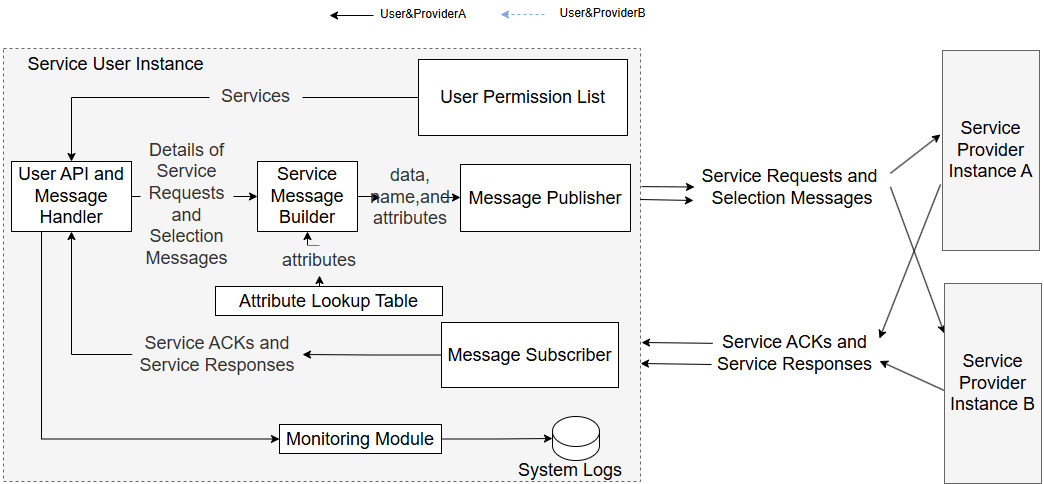
\includegraphics[width=\columnwidth]{figures/NDNSF_ServiceUser.png}
    \caption{NDNSF Service User}
    \vspace{-3mm}
    \label{fig:ServiceUser}
\end{figure}

\end{comment}

\subsection{Service Messages and Secure Communication}
\label{sec:messages}

As shown in Figure~\ref{fig:ndnsf-message-formats}, NDNSF defines four service message types---\emph{Request}, \emph{ACK}, \emph{Selection}, and \emph{Response}---each published as an NDN Data object containing a name, content, and signature. Service Users and Providers publish messages under their namespaces, announce publications through Sync, and subscribe to the messages they are responsible for processing. In the four-message flow, the Request message is one-to-many, while the remaining messages are one-to-one. The names in the figure are schematic: service names and request IDs may occupy multiple components, while an addressed participant's name occupies one encoded component.

A \textbf{Request Message} invokes a service from one or more providers. Its name follows \path{/<user>/NDNSF/REQUEST/<service>/<request-id>}, identifying the requester, the target service, and a request ID for response matching. The content includes an optional task descriptor specifying task requirements, a fresh \emph{RequestNonce}, and the provider-selection mode, all encrypted under the service attribute. Providers return the RequestNonce in subsequent ACK and Response messages to bind them to this request. The input and response keys are specific to each invocation (request-scoped protection). The task input is encrypted and delivered after selection, with its key shared only with selected providers in the Selection message.

Upon receiving a Request Message, each authorized provider decides whether to respond based on requested resources and performance requirements (Section~\ref{sec:provider-acknowledgment}). If accepted, it publishes an \textbf{ACK Message} named \path{/<provider>/NDNSF/ACK/<user>/<service>/<request-id>}. The ACK content carries the decrypted \emph{RequestNonce}, a fresh \emph{ProviderChallenge}, and optional \emph{AckMetaData}, encrypted under the permission attribute. \emph{AckMetaData} can include the number of requests in the provider's task queue or other information that may help the user select providers, e.g., resources the provider can dedicate to this request. The ACK may also identify the Provider's encryption key.

After receiving one or more ACK messages, the user issues one or more \textbf{Selection Messages} according to the provider-selection strategy (Section~\ref{sec:provider-selection}). The message name follows \path{/<user>/NDNSF/SELECTION/<provider>/<service>/<request-id>}. Its content is encrypted under the service attribute and includes a \emph{ChallengeProof} derived from the ProviderChallenge. It also carries the protected input or its Data name. The input and response keys are encrypted for the selected Provider and included in the Selection message. The Provider checks the proof and verifies that the Selection matches the request before execution.

Finally, each selected provider returns a \textbf{Response Message}, named \path{/<provider>/NDNSF/RESPONSE/<user>/<service>/<request-id>}, containing status, the protected service result or its Data name, and the \emph{RequestNonce}. The content is encrypted under the permission attribute. Decrypting the result also requires this invocation's response key; permission to read the outer message alone is insufficient. Larger input and result objects are published separately under their Producers' names.

% Addendum to the existing service-message discussion; preserve section numbering.
\label{sec:security-boundaries}
\textbf{Authorization scope and credential reuse.} ABE restricts descriptor access to entities whose DKEY policies permit decryption, including authorized providers that are not selected. Names and traffic patterns remain visible. ACK and Response content encrypted only for a service permission can also be read by other holders of that permission.

ABE policies carry service permissions, allowing baseline trust rules to focus on identity and message-signing relationships rather than per-entity service-permission lists. Identity credentials and these rules can be reused across applications sharing the same identity trust configuration. Trust rules still specify which keys may sign each message type~\cite{yu2015trust}; when processing Selection, providers must also check that it comes from the requesting user, refers to the same service and request, contains the stored provider challenge, and is allowed by the current request state. Rejecting replay requires tracking whether the request has expired or the challenge has already been used. Issuing a replacement DKEY does not invalidate an old DKEY retained by its holder. Revocation requires key rotation or additional permission checks and cannot prevent use of previously disclosed plaintext.


Table~\ref{tab:message-acceptance} summarizes the checks required by the basic invocation flow. All four message types require signature validation, an authorized signing key for the message name, and consistent service and request identifiers. The challenge checks assume that authorized participants do not disclose protected values to unauthorized parties. The invocation experiments do not independently test every rejection condition.

\begin{table*}[t]
\centering
\caption{Acceptance checks for basic invocation messages}
\label{tab:message-acceptance}
\small
\begin{tabularx}{\textwidth}{@{}lX@{}}
\toprule
Message & Additional checks before advancing the invocation \\
\midrule
Request & The provider can decrypt content protected for the requested service, and evaluates whether to participate. A duplicate request must not create a conflicting challenge or execution. \\
ACK & The user matches RequestNonce to its active request and associates the feedback and ProviderChallenge with the signing provider. Only positive ACKs passing these checks supply candidates for selection. \\
Selection & The provider matches the requesting user, service, request, and stored ProviderChallenge. The request must still permit execution, and a repeated Selection must not start a second execution. \\
Response & The user matches RequestNonce, the active request, and a selected provider. Duplicate or late results must not be accepted as results of another request. \\
\bottomrule
\end{tabularx}
\end{table*}


\subsection{Targeted Invocation}
\label{sec:targeted-invocation}

As a special case, an application that has preselected a Provider can name it in a targeted Request, for example to start a task on \texttt{drone1} or change that drone's flight-control setpoint. Targeted invocation does not substitute another device when the target is unavailable.

The Provider prepares pairs of requester and provider challenges for subsequent calls. When a valid, unused pair is available, the call can use only Request and Response; otherwise ACK and Selection must be exchanged first. The authorization, request-binding, and input-protection requirements of Section~\ref{sec:messages} still apply. Avoiding a new ACK--Selection exchange reduces repeated-call delay (Appendix~\ref{sec:targeted-invocation-evaluation}), but does not guarantee a flight-control deadline.


\subsection{Message Recovery and Timeout Handling}
\label{sec:loss-timeout}

NDNSF handles packet loss at two layers. At the synchronization and retrieval layer, NDN-SVS synchronizes publication state and retries retrieval of missing Data~\cite{moll2021svs,ndnsvs-github}. These retries aim to recover service messages without initiating a new service invocation.

At the invocation layer, NDNSF's data-driven workflow advances only when the required Data arrives and passes the applicable checks: in the four-message flow, ACK Data enables provider selection and Selection Data enables execution; Response Data delivers the result. An eligible targeted call instead uses the cached challenge material described in Section~\ref{sec:targeted-invocation} and does not wait for ACK or Selection. Request timers and, where applicable, ACK-collection timers continue to run during retrieval retries, so a recovered message may arrive too late to be used in that invocation.

If no result is accepted, the request timer triggers timeout handling. A grace interval after observed progress (500\,ms by default) and event-loop scheduling can extend acceptance beyond the configured timeout. The application decides whether to issue a new request, but a timeout does not prove that the provider did not execute the task. Retrying operations such as flight commands can therefore cause duplicate effects.

%This integrated naming, content, and encryption design ensures that NDNSF messages are not exposed to unauthorized entities while simultaneously achieving bidirectional authorization. The use of encrypted RequestNonces and one-time service tokens binds message semantics to cryptographic verification, preventing unauthorized participation and mitigating replay attacks. Even if an adversary replays previously captured messages, expired or invalid tokens will not be accepted, thereby preserving the correctness and stability of the system.

\subsection{ACK Strategy}
\label{sec:provider-acknowledgment}

In NDNSF, each provider makes a decision on whether to respond to a service request based on requested resources and performance requirements. The requested resources may include CPU/GPU, memory, trusted execution environments, and bandwidth. Performance requirements may further include response time and computation accuracy level. A provider publishes a positive ACK when its application-defined strategy accepts the task; this reports willingness to participate, without reserving resources or guaranteeing that the requirements will still be met when execution begins.
%This mechanism mitigates resource exhaustion, reduces unnecessary waiting time, and improves system stability. 

\subsection{Provider Selection Strategy}
\label{sec:provider-selection}

\begin{figure}
    \centering
    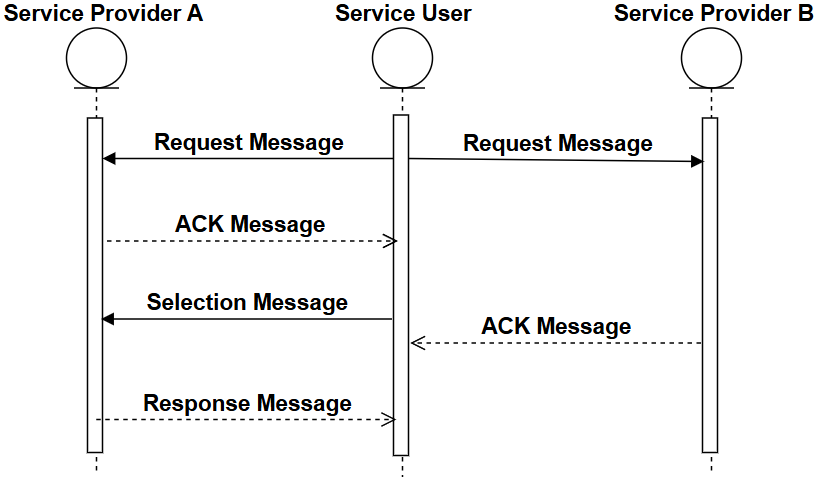
\includegraphics[width=.9\columnwidth]{figures/First-Responding.png}
    \caption{First-Responding Strategy}
    \label{fig:First-Responding}
\end{figure}

\begin{figure}
    \centering
    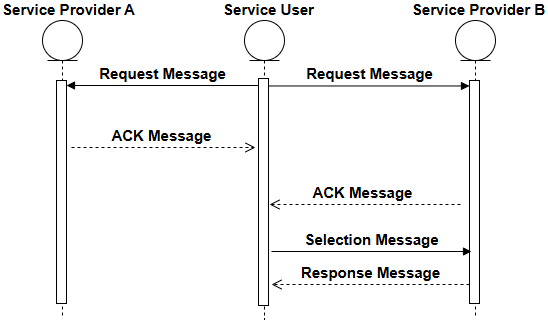
\includegraphics[width=.9\columnwidth]{figures/Random-Selection.png}
    \caption{Random-Selection Strategy}
    \label{fig:Random-Selection}
\end{figure}

\begin{figure}
    \centering
    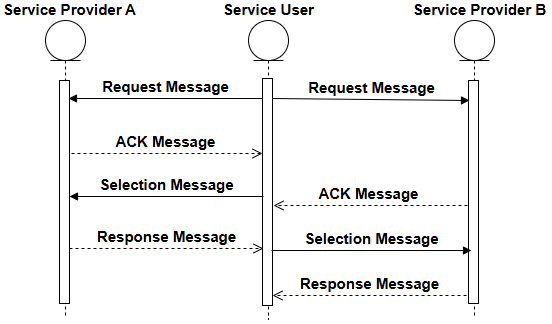
\includegraphics[width=.9\columnwidth]{figures/All-Responders.png}
    \caption{All-Responders Strategy}
    \label{fig:All-Responders}
\end{figure}

When multiple service providers offer the same service, NDNSF enables the user to select one or more providers for execution. It supports three built-in provider selection strategies, as well as user-defined custom strategies, allowing optimization based on metrics such as RTT, computational capacity, bandwidth, or other application-specific requirements. Candidates must return positive ACKs that pass the applicable message and authorization checks.
\begin{enumerate}
\item \textbf{First-Responding Strategy (Figure~\ref{fig:First-Responding})}: the user selects the first provider that returns a valid ACK. For example, if Drone~1 and Drone~2 both offer the \texttt{YOLO12} service and Drone~1 responds first, Drone~1 is selected.
\item \textbf{Random-Selection Strategy (Figure~\ref{fig:Random-Selection})}: when the ACK-collection window closes, the user randomly selects one provider from the collected valid ACKs. This is suitable for load balancing among similar providers.
\item \textbf{All-Responders Strategy (Figure~\ref{fig:All-Responders})}: all providers whose valid ACKs are collected before the window closes are selected to execute the service. This is intended for redundancy or cross-validation, e.g., multiple drones independently sensing the same target.
\item \textbf{Custom-Selection Strategy}: NDNSF also supports user-defined provider-selection strategies based on published service information, application-supplied runtime measurements, and optional metadata included in ACK messages by providers (e.g., resource availability and processing cost).
\end{enumerate}
For strategies that collect ACKs, the window may close early when the reply count reaches the recently observed provider count, reducing wait while excluding later ACKs.
\subsection{NDNSF Application Programming Interface}
\label{sec:NDNSF-API}

\begin{figure}[]
\centering

% --- Top Listing: Provider-Side API ---
\begin{lstlisting}[
    style=ndnsfstyle,
    language=C++,
    caption={Provider-Side API},
    label={lst:provider-api}
]
void Provider::addService(
    ServiceName service,
    AckHandler onAck,
    RequestHandler onRequest
);
\end{lstlisting}

\vspace{4mm} % Adds a clean breathing gap between the two blocks

% --- Bottom Listing: User-Side API ---
\begin{lstlisting}[
    style=ndnsfstyle,
    language=C++,
    caption={User-Side API},
    label={lst:async-call}
]
RequestId User::RequestService(
    ServiceName service,
    RequestPayload request,
    int ackCollectionTimeMs,
    AckSelectionPolicy selectionPolicy,
    int timeoutMs,
    ResponseCallback onResponse,
    TimeoutCallback onTimeout
);
\end{lstlisting}

\caption{Simplified APIs for the four-message invocation flow}
\label{fig:ndnsf-apis}
\end{figure}

Figure~\ref{fig:ndnsf-apis} summarizes the invocation API using simplified types.

%LW: does the provider call this only one time for all the incoming requests
\texttt{addService} registers a named service together with two callbacks, \texttt{onAck} and \texttt{onRequest}. In the four-message flow, the \texttt{onAck} callback is invoked when a request is received, allowing the provider to decide whether to serve the request and optionally include metadata in its ACK. The \texttt{onRequest} callback is invoked after the user selects the provider and sends a Selection message; an eligible targeted call can reach execution without a new Selection exchange. This two-stage flow enables informed decision making by both providers and users.

%LW: what if there are multiple responses?
\texttt{RequestService} is the primary user-side service invocation interface. The application specifies the service name and request payload, without explicitly identifying providers. It also supplies two timeout values, a \texttt{selectionPolicy}, and two callbacks, \texttt{onResponse} and \texttt{onTimeout}. NDNSF publishes the request to solicit eligible providers and uses \texttt{ackCollectionTimeMs} to configure the ACK-collection window. It applies the policy as ACKs arrive or when the window closes. Accepted responses are delivered to \texttt{onResponse}; request expiration is handled by \texttt{onTimeout} as described in Section~\ref{sec:loss-timeout}.

For a service registered to support targeted invocation, \texttt{RequestServiceTargeted} takes the provider name, service name, request, timeout and timeout/response callbacks. The application supplies the target; the framework applies the authorization checks and challenge-pair rules described in Section~\ref{sec:targeted-invocation}.
